% !TeX spellcheck = en_GB

\section{DWH Implementation}

\begin{breakbox}
\boxtitle{MOLAP:}
\newline Multi-dimensional OLAP stored in n-dimensional arrays.
\begin{center}
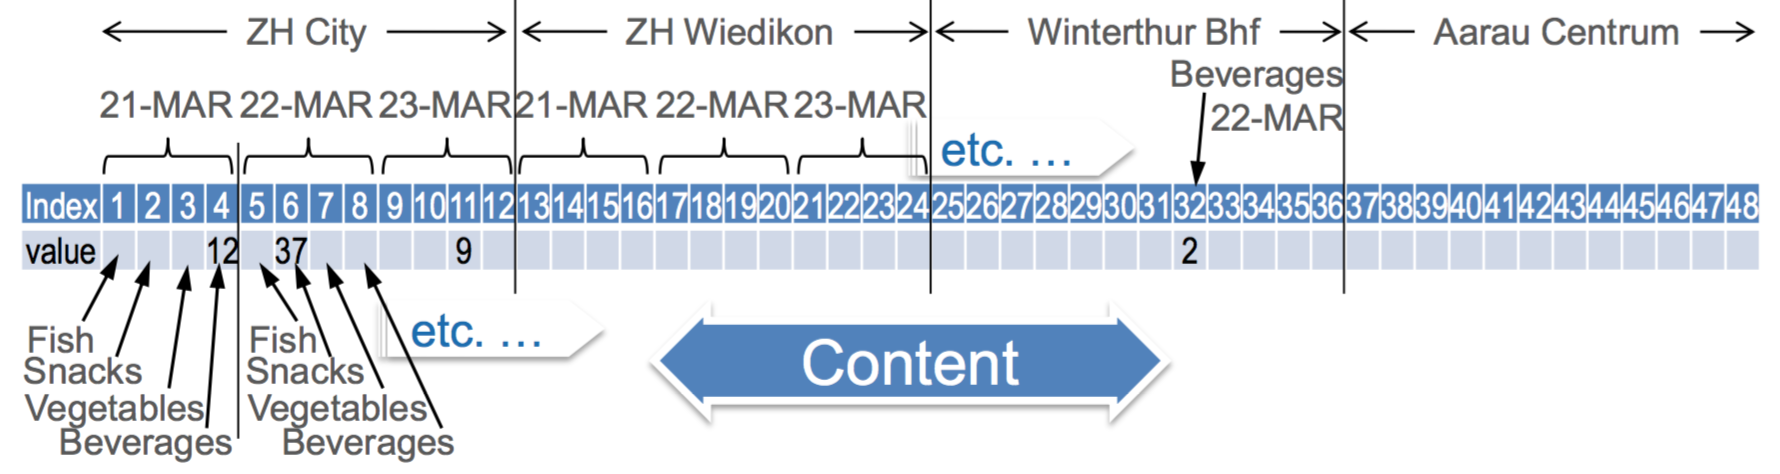
\includegraphics[width=.15\textwidth]{slides_images/molap}
\end{center}
Formula for storage (and query):
\begin{center}
$i_{1k} + (i_{2l}-1) \cdot |I_1| + (i_{3m}-1) \cdot |I_1| \cdot |I_2| + \cdots$,
\end{center}
with $I_j =$ dimension $j$, $i_{jk} =$ index for $k^{th}$ element of dimension $j$.
\end{breakbox}

\begin{breakbox}
\boxtitle{Example (Pages):}
\newline Following tables and data are given. Dimensions are ordered as follows: shipment, supplier, year, product.
\begin{center}
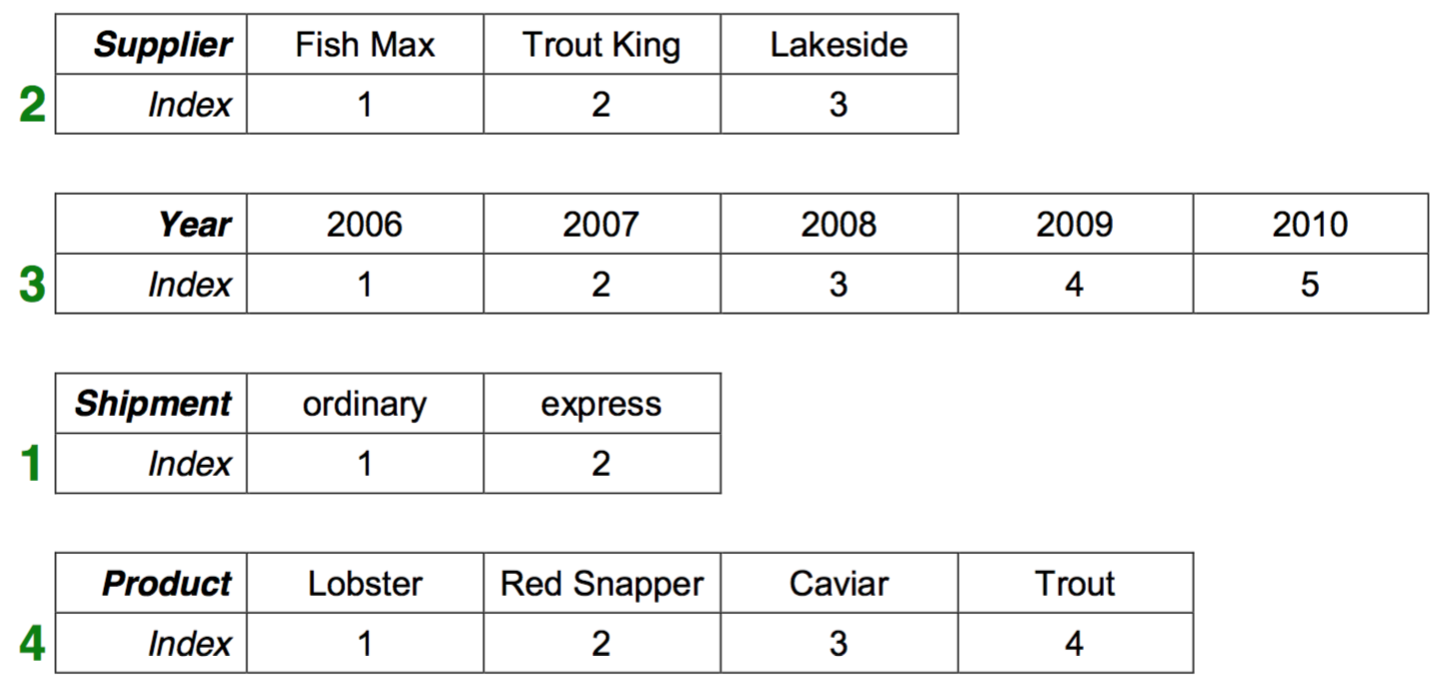
\includegraphics[width=.15\textwidth]{slides_images/molap_example}
\end{center}
Exercise: A page can hold 4 array cells.
\begin{enumerate}[label=(\alph*)]
	\item How many pages have to be loaded for a query after all sales of Lobster in 2008?
		\begin{itemize}
			\item[] All Lobster array cells adjacent (since it's last dimension in order). Lobster in 2008 spreads over 6 cells (all combinations from Supplier and Shipment dimensions). 6 / 4 = 2 pages.
		\end{itemize}
	\item How many pages have to be loaded for a query after all sales by express in 2008?
		\begin{itemize}
			\item[] The 2008 and express combinations spread over 5 cells (i.e. 2 pages), but there are several of those ranges , dispersed over Lobster, Red Snapper, Caviar and Trout. So 4 x 2 = 8 pages.
		\end{itemize}
\end{enumerate}
\begin{center}
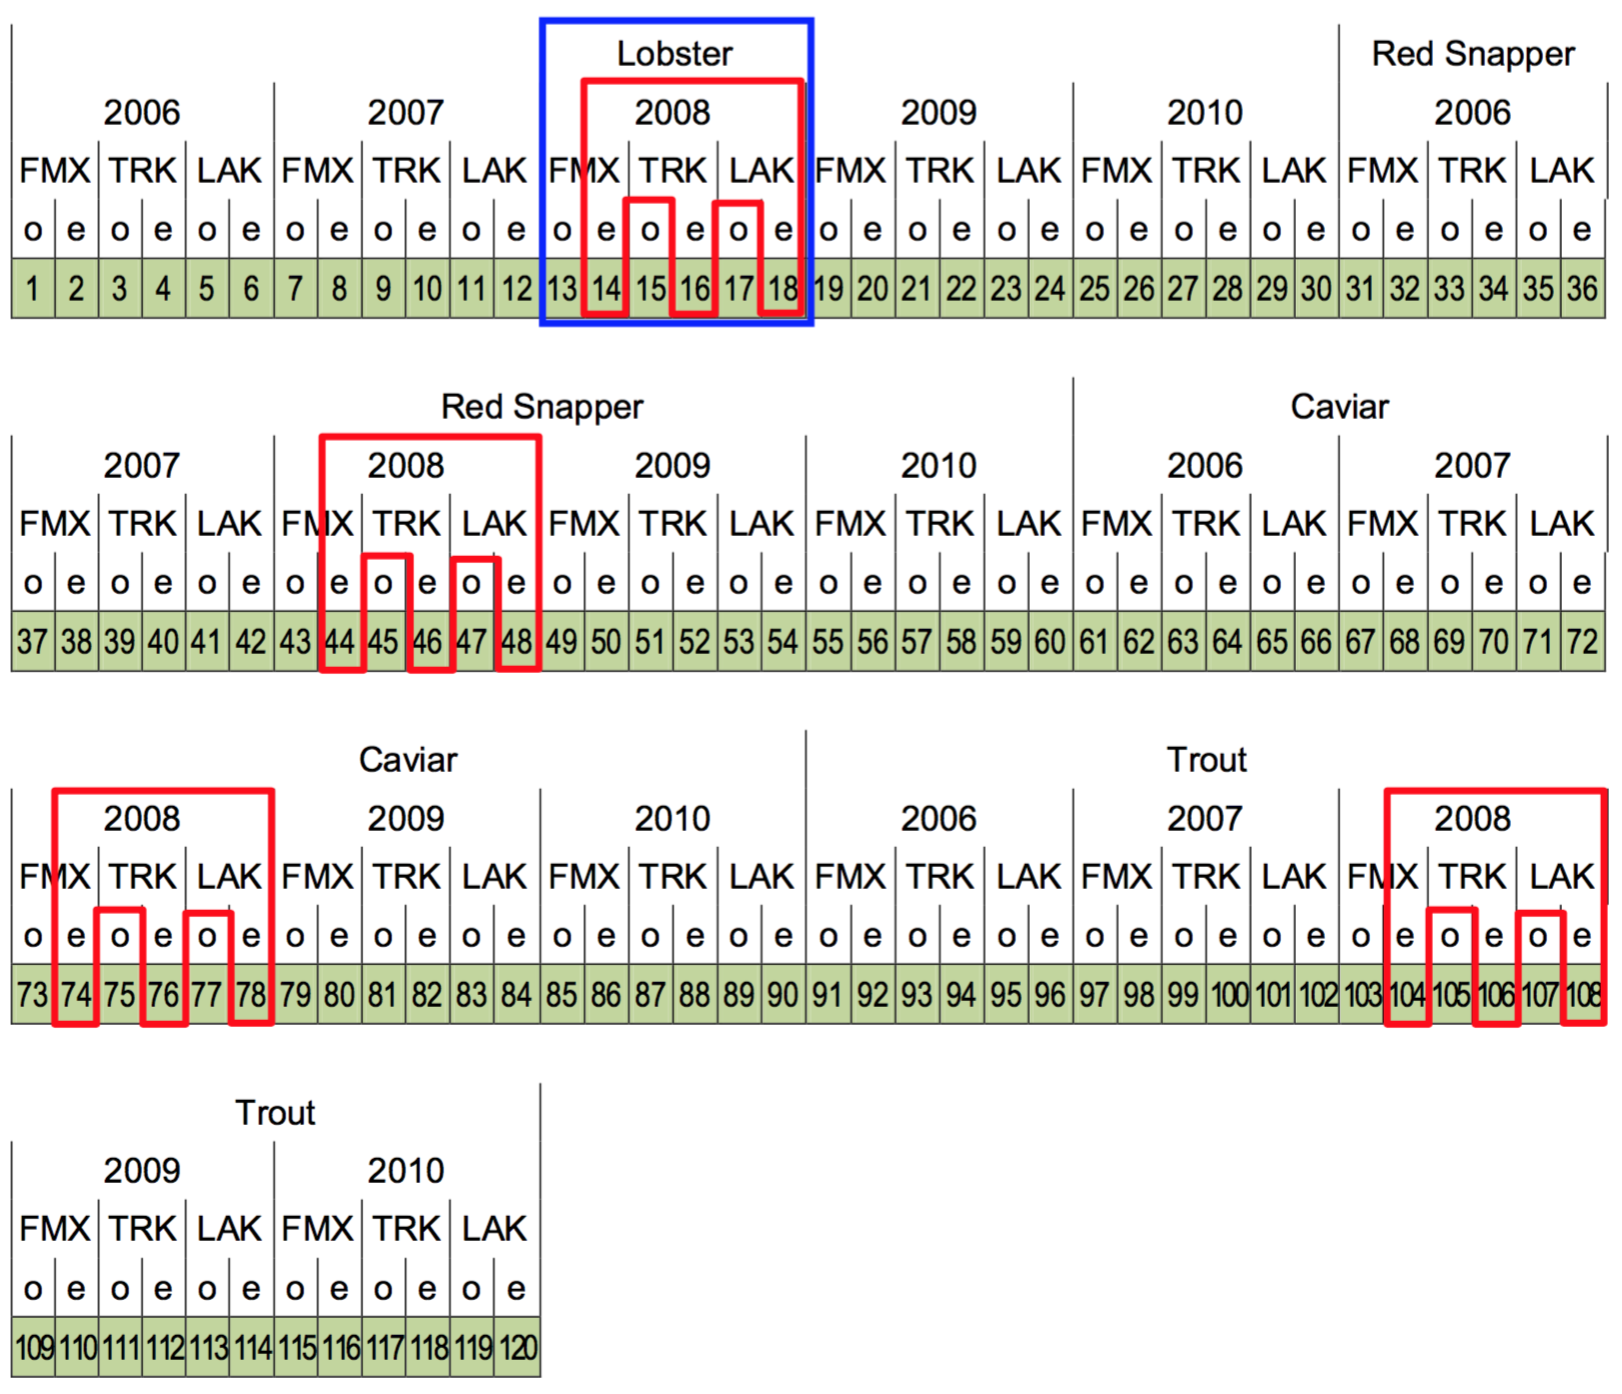
\includegraphics[width=.15\textwidth]{slides_images/molap_solution}
\end{center}
\end{breakbox}

\begin{breakbox}
\boxtitle{FASMI:}
Trying to define OLAP
\begin{itemize}
	\item \textcolor{Emerald}{F}ast: response time < 5 s, complex queries max. 20 s.
	\item \textcolor{Emerald}{A}nalysis: intuitive analytical functionality.
	\item \textcolor{Emerald}{S}hared: more than 1 user, authorization, authentication.
	\item \textcolor {Emerald}{M}ultidimensional: Multidimensional conceptual view on data.
	\item \textcolor{Emerald}{I}nformation: analysis not limited by OLAP system.
\end{itemize}
\end{breakbox}
\begin{breakbox}
\boxtitle{Optimize MOLAP:}
\newline To address data sparsity MOLAP implementation usually differentiates between:
\begin{itemize}
	\item dense dimensions (e.g. Time, Location, Salesperson).
	\item sparse dimensions (e.g. Customer, Product, Sales Promotion).
	\item dense dimensions form a data block.
	\item sparse dimensions are kept as indexes.
	\item data blocks only exist where sparse dimensions hold values.
\end{itemize}
\begin{center}
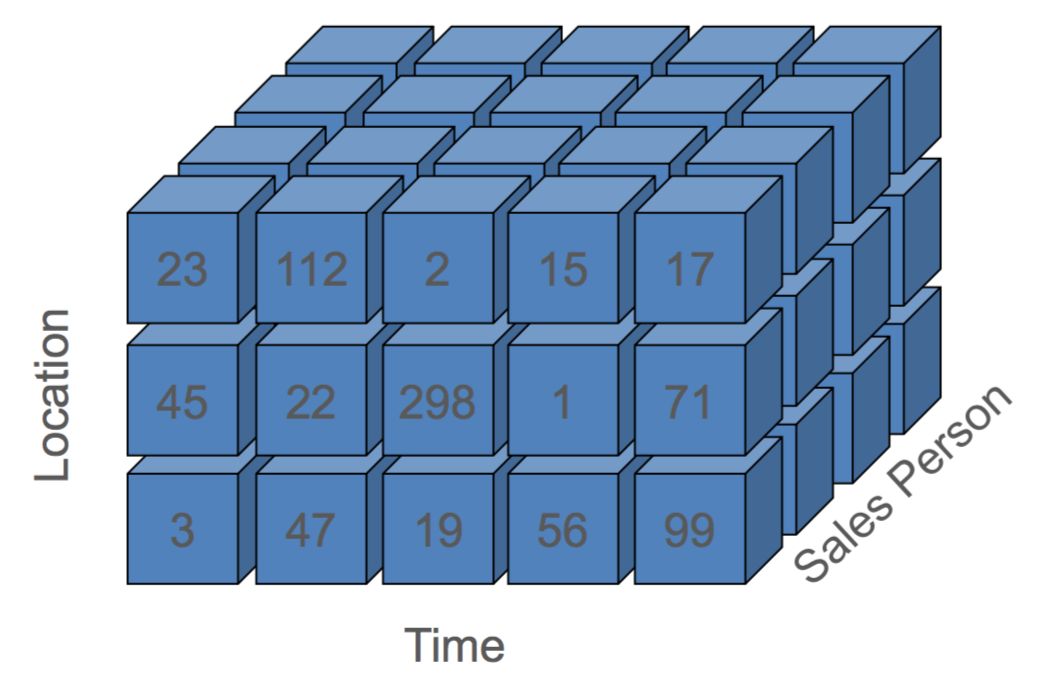
\includegraphics[width=.05\textwidth]{slides_images/dense_molap}
\end{center}
\begin{itemize}
	\item data block
	\begin{itemize}
		\item containing individual array cells.
		\item for relatively dense dimensions.
	\end{itemize}
\end{itemize}
\begin{center}
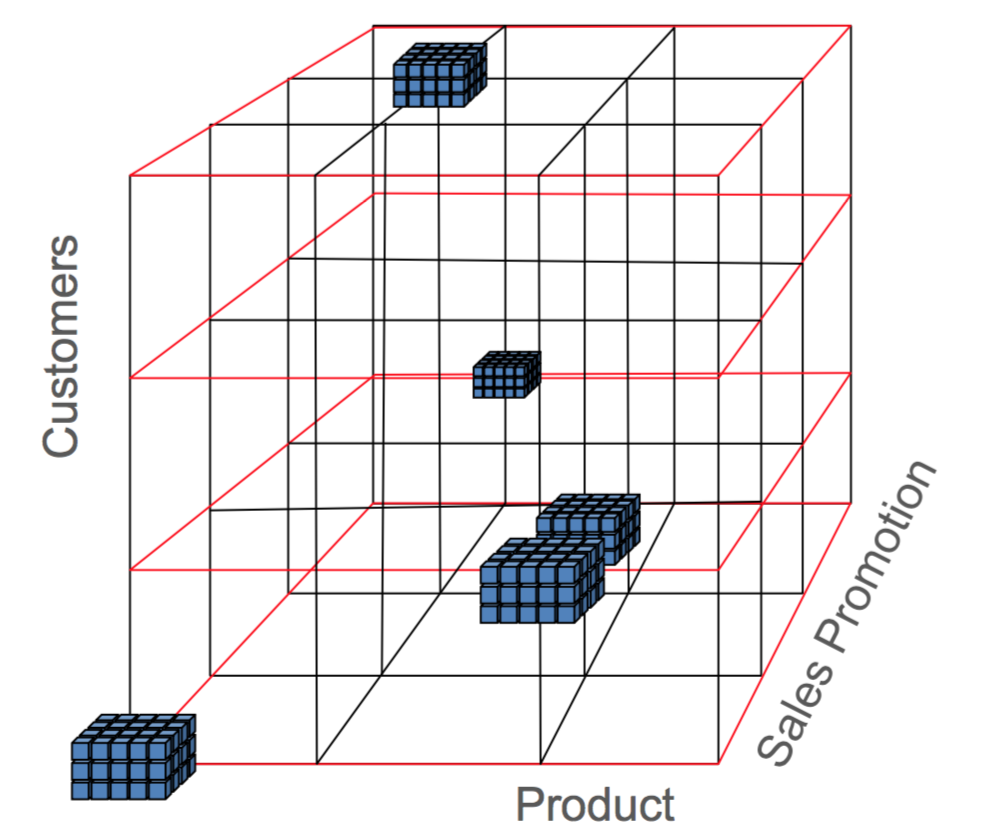
\includegraphics[width=.05\textwidth]{slides_images/sparse_molap}
\end{center}
\begin{itemize}
	\item data blocks are only stored for actual occurrences in sparse dimensions.
\end{itemize}
\end{breakbox}

\begin{breakbox}
\boxtitle{MOLAP vs. OLAP:}
\newline MOLAP:
\begin{itemize}
	\item faster computation.
	\item efficiency sensitive to increase in data volume and dimensions.
\end{itemize}
ROLAP:
\begin{itemize}
	\item larger amounts of data.
	\item scalability.
	\item mature DBMSs (concurrency, data management, recovery $\ldots$).
	\item constant transformation necessary between multidimensional $\leftrightarrow$ relational model.
\end{itemize}
\end{breakbox}

\begin{breakbox}
\boxtitle{HOLAP:} Hybrid approach between MOLAP and ROLAP.
\begin{itemize}
	\item sparse data remains in relational DB.
	\item dense data gets exported to multidimensional arrays.
\end{itemize}
Advantage of arrays over relations:
\begin{itemize}
	\item depends on allocation rate of data in cube.
	\item starts at certain thresholds.
\end{itemize}
\end{breakbox}

\begin{breakbox}
\boxtitle{Optimize ROLAP:}
\newline RDBS performance: suffers most from joins of huge data sets.
\newline Optimization objective: significantly reduce data sets by indexing.
\newline Special indexes often applied with DWHs:
\begin{description}
	\item[Join Indexes] Index pointing on multiple tables.
	\item[Bitmap Indexes] A bitvector for each indexed attribute with a 
	bitvector for each distinct value (bit=1 value occurs, else 0).
\end{description}
\end{breakbox}

\begin{breakbox}
\boxtitle{Join Indexes:}
\begin{center}
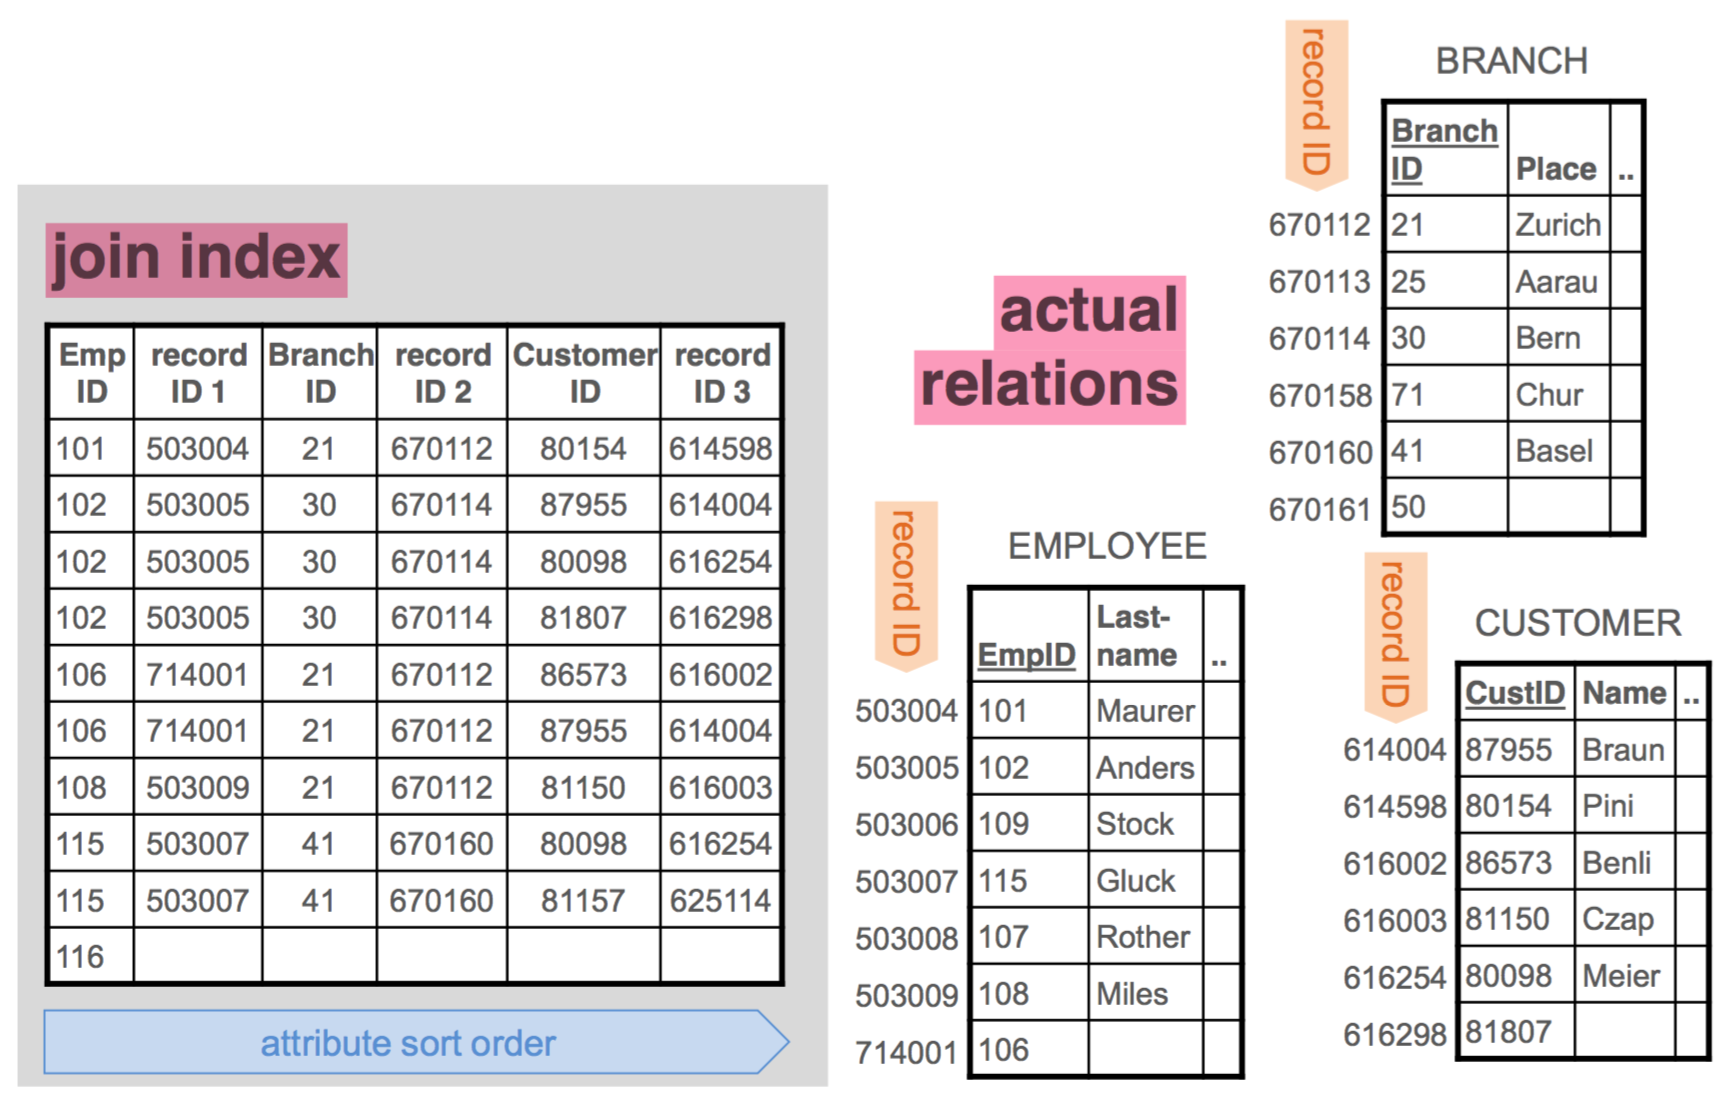
\includegraphics[width=.15\textwidth]{slides_images/join_indexes}
\end{center}
\begin{itemize}
	\item combine record IDs for attributes in multiple tables at a time.
	\item create indexes for every such attribute combination frequently used for joins
	\begin{itemize}
		\item e.g. dimension attributes
		\item combinational explosion!
	\end{itemize}
	\item sort order of attributes impacts query acceleration.
\end{itemize}
\end{breakbox}

\begin{breakbox}
\boxtitle{ETL:}
\newline \textcolor{Emerald}{E}xtraction, \textcolor{Emerald}{T}ransforming and \textcolor{Emerald}{L}oading.
\end{breakbox}

\begin{breakbox}
\boxtitle{Extraction:}
\newline Capture data in operational systems:
\begin{itemize}
	\item risk of interference with everyday business transactions.
\end{itemize}
Physical extracts:
\begin{itemize}
	\item for performance reasons.
	\item risk of losing hard coded information, e.g. pointers representing relationships.
\end{itemize}
Not all data is extracted:
\begin{itemize}
	\item selection specific to later analytical needs.
\end{itemize}
What data looks like:
\begin{itemize}
	\item lacking (not recorded, not entered).
	\item contradictory (different understanding, e.g.
in different source systems).
	\item on different scales.
	\item redundancy.
	\item noisy (random irregularities).
	\item errors.
	\item only aggregated values available.
\end{itemize}
\end{breakbox}

\begin{breakbox}
\boxtitle{Transformation:}
\newline i.e. data consolidation:
\begin{itemize}
	\item achieve a general level of data quality (across all source database systems)
\end{itemize}
No 1:1 copy of operational data:
\begin{itemize}
	\item aggregation
	\item filtering
	\item restructuring and reformatting
	\item completion
	\item adding remarks
\end{itemize}
\end{breakbox}

\begin{breakbox}
\boxtitle{Loading:}
\newline Move into DWH:
\begin{itemize}
	\item sometimes preformatted to physical format.
\end{itemize}
Integrity checks
\begin{itemize}
	\item before load
	\item after load with respect to data already in DWH, e.g. for uniqueness.
\end{itemize}
Build indexes:
\begin{itemize}
	\item time consuming
	\item insert $\leftrightarrow$ drop and rebuild
\end{itemize}
\end{breakbox}
